\documentclass[12pt]{article}
\usepackage[english]{babel}
\usepackage{amsmath,amsthm}
\usepackage{graphicx}
\usepackage{caption}
\usepackage{subcaption}
\usepackage{amsfonts}
\usepackage{indentfirst}
\usepackage{lscape}
\usepackage[top=2.5cm,bottom=2.5cm,right=2.5cm,left=2.5cm]{geometry}
\usepackage{titlesec}
\setcounter{secnumdepth}{5}

% ----------------------------------------------------------------
\begin{document}

\section{Results}

In this part, we will present the result we obtained in this project. We divide this section in two subsections, the first is the procedure we use for testing our descriptors. And the second is the presentation of the results and the comparison of the two descriptors.

\subsection{Procedure}

\subsubsection{For one image}
In a first place, we use the result of the K-means for classify one image taking training database as reference:

\begin{figure}[h]
    \center
    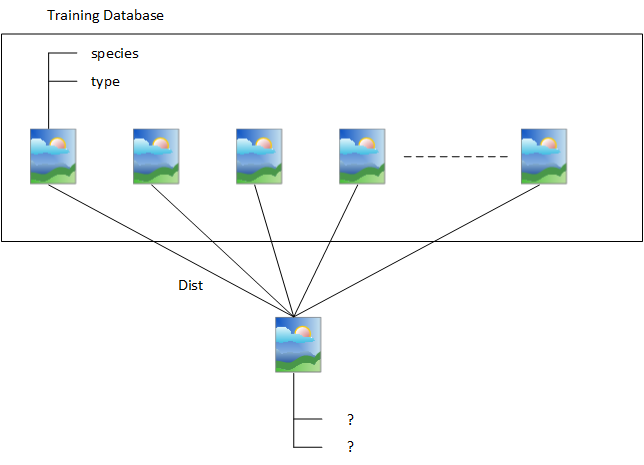
\includegraphics[scale=0.95]{proced.png}
    \caption{Classification for one picture}\label{fig:proced1}
\end{figure}

For the SIFT descriptor we will compare the Euclidean distance \eqref{Disteuclid} and the $\chi^2$ distance \eqref{Distki}. The comparison of these distances in the C$_2$O algorithm is made in the K-means algorithm.

After the distance calculation we use the K-nn algorithm to find the species of the picture.

\begin{equation}
T_{E}(H^1,H^2) = \sqrt{\sum_{i=1}^{n} (h_{i}^{1} - h_{i}^{2})^2}
\label{Disteuclid}
\end{equation}

\begin{equation}
T_{\chi^2}(H^1,H^2) = \sum_{i=1}^{n} \frac{(h_{i}^{1} - h_{i}^{2})^2}{(h_{i}^{1} + h_{i}^{2})^2}
\label{Distki}
\end{equation}

\vspace{2cm}

\subsubsection{For a database}
For a database we use the same method that we use for one image. For the treatment of a database we can use two different method:

\begin{itemize}
\item cross-classification 

\begin{figure}[h]
    \begin{minipage}{0.50\linewidth}
        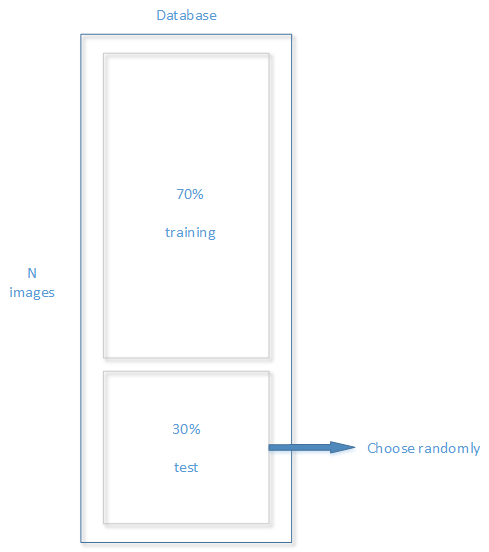
\includegraphics[scale=0.7]{proced2.png}
        \caption{Classification for a database}\label{fig:proced2}
    \end{minipage}\hfill
    \begin{minipage}{0.55\linewidth}
        The difference is that we will take 80\% of the images as a training base, and 20\% as test. The 20\% are choose randomly, but to have a means of the whole database result, we will iterate this process, and the signature of the images choose at the previous iteration can not be in the 20\% of test.
    \end{minipage}
\end{figure}

\newpage
\item let

\begin{figure}[h]
    \begin{minipage}{0.50\linewidth}
        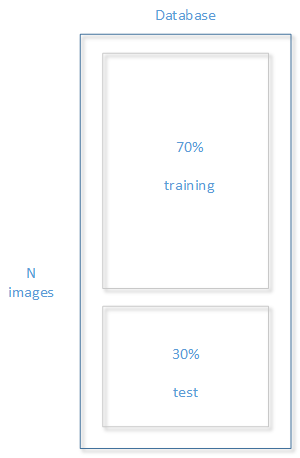
\includegraphics[scale=0.7]{proced3.png}
        \caption{Classification for a database}\label{fig:proced3}
    \end{minipage}\hfill
    \begin{minipage}{0.55\linewidth}
        In this second method, we choose the same training base (70\% of the database), and the same test base (30\% of the database). This method allows us to see the difference between two different distance, or between the SIFT and the C$_2$O.
    \end{minipage}
\end{figure}

\end{itemize}

In scope of respecting our project schedule we have to present results so we will use the second method to have results to compare. 

\subsection{Analysis of result}

% ----------------------------------------------------------------
\end{document} 
